\documentclass{thesis}

\title{Data Storage and Serving Architecture for HTRC Corpus}
\author{HTRC IU Team}

\begin{document}

\maketitle

\tableofcontents

\begin{abstract}
TBD.
\end{abstract}

\section{Introduction}
With the recent acquisition of full Hathitrust corpus of 13.8 million digitized volumes, HTRC is working towards providing non-consumptive access to the full corpus. HTRC stores the corpus in IU Data Capacitor 2 structured according to pairtree~\cite{pairtree} file system heirarchy. Also, there is a copy of pairtree content packed into binary blobs that work with a in-house data processing and serving solution for HPC.

Data Capsules enable non-consumptive access to HTRC corpus and HTRC serves data to Data Capsules via the Data API~\cite{dataapi} which is a REST service backed by a Cassandra cluster. Current Data API provides access to a part of the full corpus, which is about 4 million digitized volumes.

HTRC aims to provide non-consumptive access to full Hathitrust corpus in coming months and this document discusses requirements and solutions for enabling non-consumptive access to full corpus efficiently.

\section{Requirements}

\begin{itemize}
	\item Serve the full corpus via a REST API
	\item Provide page level access
	\item Ability achieve high throughputs to sufficiently utilize 40Gb/s network link
	\item HTRC Data SDK
	\item Enable processing the corpus using Big Data frameworks such as Hadoop and Spark
\end{itemize}
    

\section{Discussion Notes}

\begin{figure}[ht!]
    \centering
    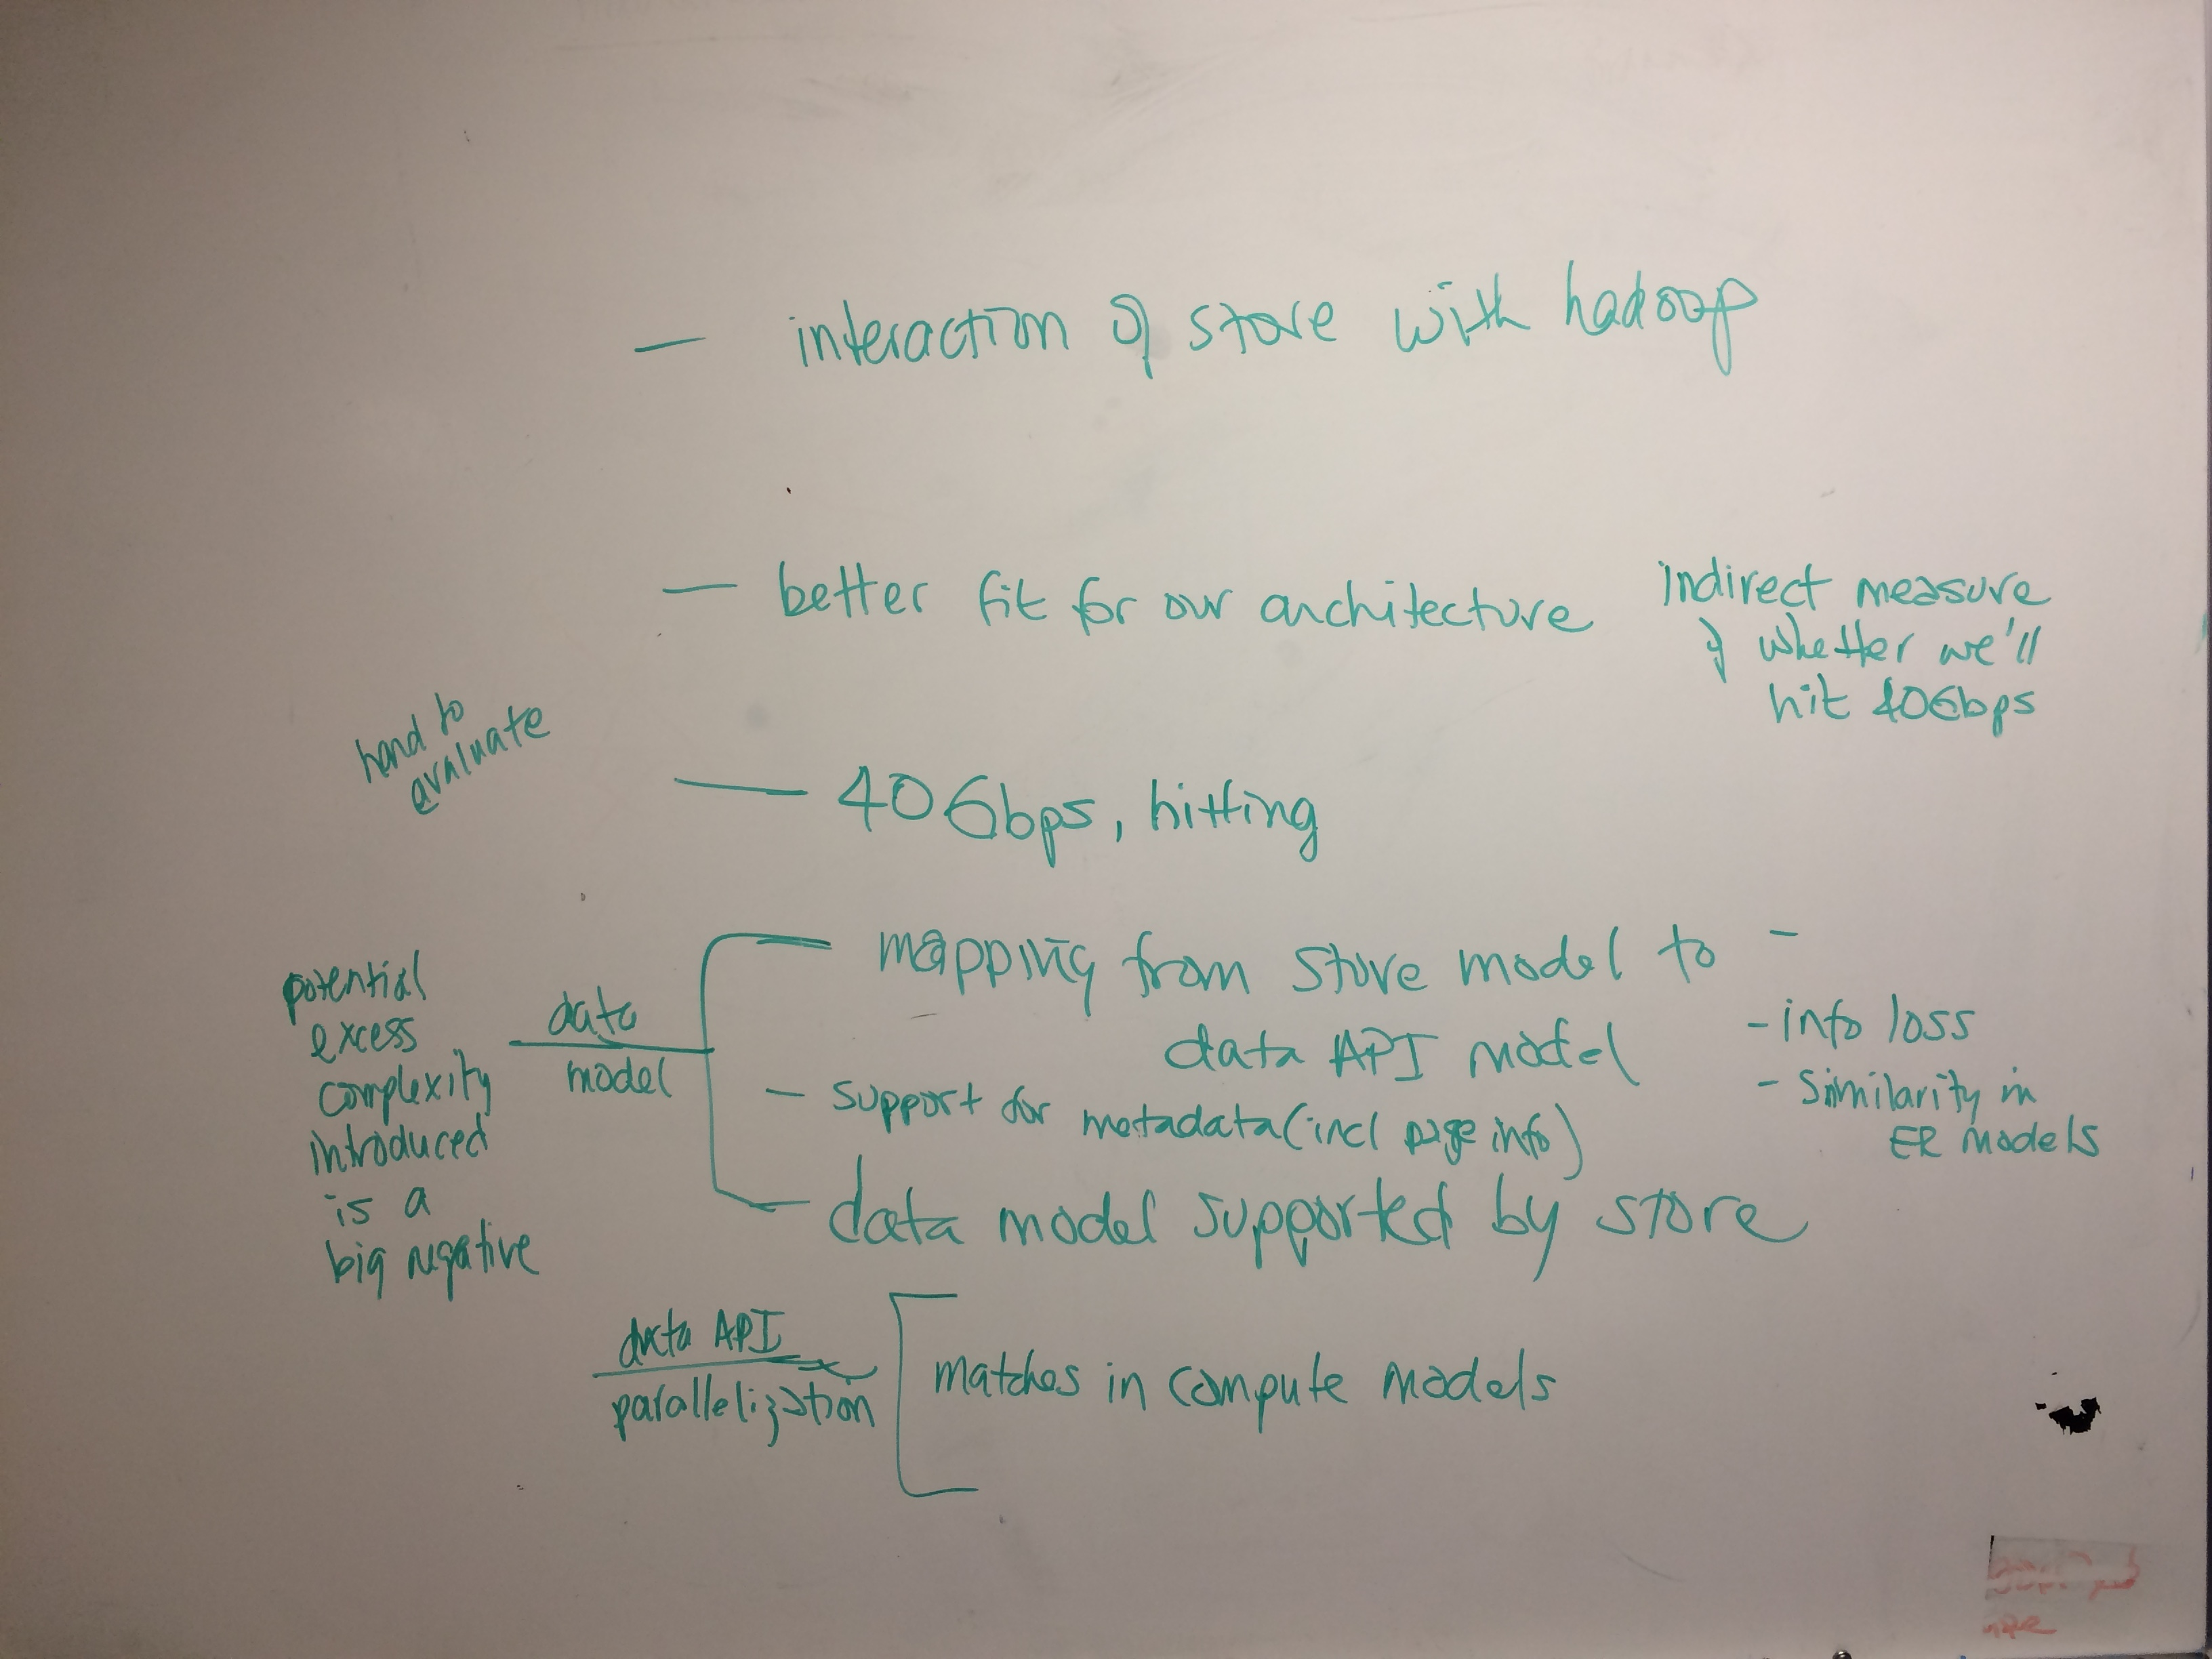
\includegraphics[width=0.95\textwidth]{IMG_0475}
    \caption{Notes from the July 13th discussion (Milinda and Beth)}
    \label{fig:notes}
\end{figure}


\bibliographystyle{abbrv}
\bibliography{references}

\end{document}